\subsection{Posições Chave}\label{subsec:pos_chave}

Devido ao grande número de possibilidades para as posições dos robôs,
somente a geração de posições aleatórias não gera bons resultados
para as ações do tipo $Mover(r_i)$. Portanto, para direcionar a busca,
foi desenvolvida uma maneira de se sugerir posições para as ações em
questão com o auxílio da interface gráfica.
A Figura~\ref{fig:pos_chave_barreira} mostra a sugestão de uma barreira.
Já na Figura~\ref{fig:pos_chave_lateral} são sugeriadas posições laterais. 

\begin{figure}[H]
  \centering
  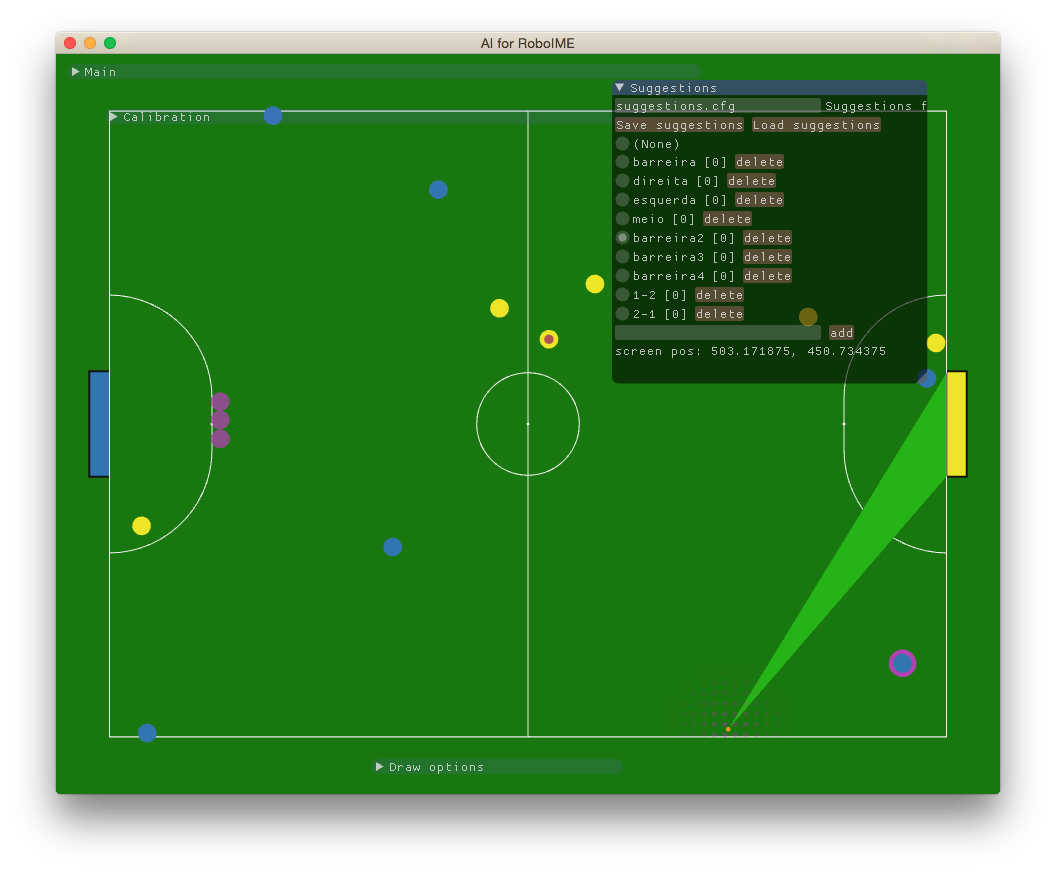
\includegraphics[width= 0.8\linewidth]{pos_chave_barreira}
  \caption{Sugestão de uma barreira (em rosa)}\label{fig:pos_chave_barreira}
  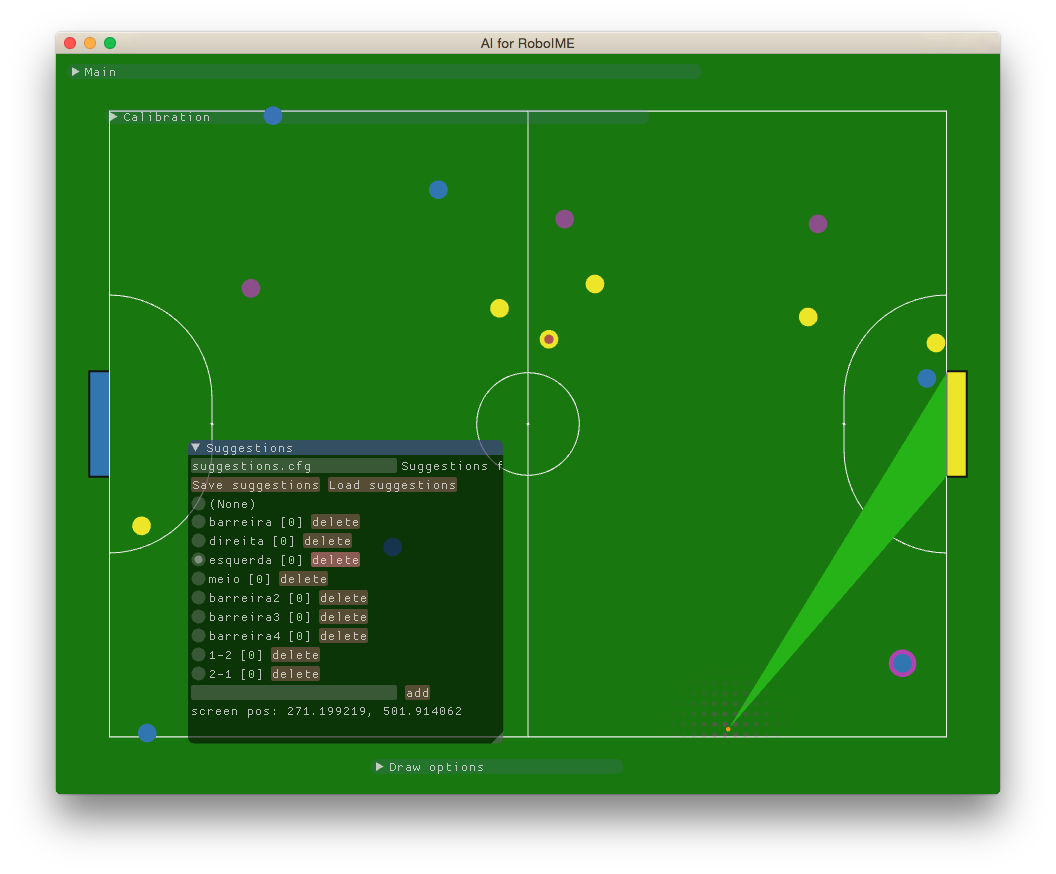
\includegraphics[width= 0.8\linewidth]{pos_chave_lateral}
  \caption{Sugestão de posições laterais (em rosa)}\label{fig:pos_chave_lateral}
\end{figure}

Com o objetivo de verificar a utilidade das posições chave,
foi criada uma maneira de identificar se uma posição chave
foi utilizada.

As posições chave são utilizadas das seguinte maneira:
\begin{itemize}
  \item Caso um número de posições inferior ao número de
        robôs sejam sugeridas, são criadas ações aleatórias
        para completar a sugestão.
  \item As posições sugeridas são atribuidas para o robô
        mais próximo da posição sugerida. Isso é feito
        na ordem em que as posições foram sugeridas
\end{itemize}

% vim: tw=80 et ts=2 sw=2 sts=2 ft=tex
